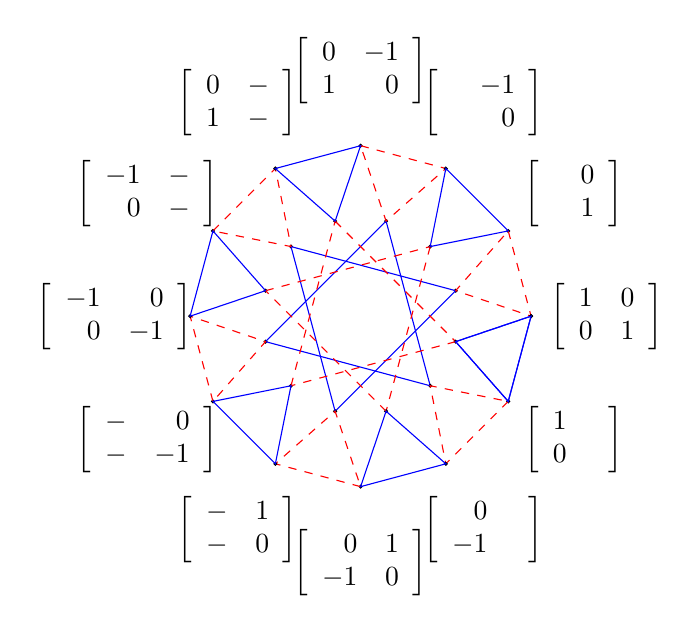
\begin{tikzpicture}[scale=1.25]
  \foreach \x in {15,75,...,330} {
    \filldraw[black] (\x:1cm) circle(0.4pt); % dots at each point
    % lines across inside
    \draw[blue] (\x:1cm) -- (\x-120:1cm);
  }
  \foreach \x in {45,105,...,345} {
    \filldraw[black] (\x:1cm) circle(0.4pt); % dots at each point
    % lines across outside
    \draw[red,dashed] (\x:1cm) -- (\x-120:1cm);
  }
  \foreach \x in {30,90,...,330} {
    \filldraw[black] (\x:1.73205cm) circle(0.4pt); % dots at each point
    % lines across inside
    \draw[red,dashed] (\x:1.73205cm) -- (\x-30:1.73205cm) -- (\x-15:1cm) -- cycle;
  }
  \foreach \x in  {0,60,...,360} {
    \filldraw[black] (\x:1.73205cm) circle(0.4pt); % dots at each point
    % lines across inside
    \draw[blue] (\x:1.73205cm) -- (\x-30:1.73205cm) -- (\x-15:1cm) -- cycle;
  }
  \foreach \x/\a/\b/\c/\d in {
    0/1/0/0/1,
    30/\ow/0/\w/1,
    60/\ow/-1/\w/0,
    90/0/-1/1/0,
    120/0/-\ow/1/-\w,
    150/-1/-\ow/0/-\w,
    180/-1/0/0/-1,
    210/-\ow/0/-\w/-1,
    240/-\ow/1/-\w/0,
    270/0/1/-1/0,
    300/0/\ow/-1/\w,
    330/1/\ow/0/\w
  }
  \draw (\x:2.5cm) node { $\left[ \begin{array}{rr} \a & \b \\  \c & \d \end{array}\right]$};      
\end{tikzpicture} 
